% !TEX program = lualatex
% ECON 201, Worksheet 22: Regulation, Taxes, and Compensation.
% Compile with LuaLaTeX so the PDF is tagged. Build from the course root:
%   latexmk -lualatex -cd worksheets/worksheet22.tex && latexmk -c -cd worksheets/worksheet22.tex
% Every number here is computed and printed by slides/figures/make_worksheet22.py
% (a warehouse next to a neighborhood, truck trips a day; its own example,
% different from the deck's banana island; the script also draws
% figures/warehouse-grid.pdf).
\DocumentMetadata{
  pdfstandard=UA-2,
  pdfversion=2.0,
  lang=en-US,
  tagging=on
}
\documentclass[11pt]{article}

\usepackage[letterpaper, margin=0.75in, top=0.45in, bottom=0.4in]{geometry}
\usepackage{fontspec}
\setmainfont{Fira Sans}
\usepackage{amsmath}
\usepackage{amssymb}
\usepackage{graphicx}
\usepackage{booktabs}
\usepackage{array}
\usepackage{xcolor}
\usepackage{needspace}
\usepackage[most]{tcolorbox}
\definecolor{cream}{HTML}{FDF3EA}
\definecolor{accent}{HTML}{BF5700}
\usepackage{titlesec}
\titleformat{\section}{\large\bfseries\color{accent}}{}{0pt}{}
\titlespacing*{\section}{0pt}{4pt}{2pt}
\usepackage{hyperref}
\hypersetup{pdftitle={ECON 201 Worksheet: Regulation, Taxes, and Compensation}, pdfauthor={Div Bhagia}, hidelinks}
\pagestyle{empty}
\setlength{\parindent}{0pt}
\setlength{\parskip}{2pt}

% Ruled answer space: n lines. Plain TeX loop; pgffor's \foreach breaks the
% enumerate counter when used inside an item.
\newcount\answerlinecount
\newcommand{\answerlines}[1]{%
  \par\vspace{1pt}\answerlinecount=#1
  \loop\ifnum\answerlinecount>0
    \rule{\linewidth}{0.3pt}\par\vspace{5pt}%
    \advance\answerlinecount by -1
  \repeat
  \vspace{-5pt}}

\begin{document}

{\LARGE\bfseries\color{accent} Worksheet: Regulation, Taxes, and Compensation}\hfill{\large ECON 201}

% Terms sit on the cream panel, where the brand orange falls below 4.5:1;
% the darker orange keeps WCAG AA contrast (see CLAUDE.md).
\definecolor{accentdark}{HTML}{8F4100}
\newcommand{\term}[1]{\textcolor{accentdark}{\textbf{#1}}}

% Definitions panel list: flush left, compact (see worksheet09).
\newenvironment{deflist}
  {\begin{list}{\textbullet}{%
     \setlength{\leftmargin}{1.1em}\setlength{\labelwidth}{0.7em}%
     \setlength{\labelsep}{0.4em}\setlength{\itemindent}{0pt}%
     \setlength{\listparindent}{0pt}\setlength{\topsep}{2pt}%
     \setlength{\partopsep}{0pt}\setlength{\parsep}{0pt}%
     \setlength{\itemsep}{2pt}}}
  {\end{list}}

\begin{tcolorbox}[colback=cream, colframe=accent, boxrule=0.6pt, arc=2pt,
  left=6pt, right=6pt, top=4pt, bottom=4pt, title=Definitions,
  fonttitle=\bfseries, coltitle=white]
\begin{deflist}
\item \term{Marginal private cost (MPC)}: the firm's own cost of one more unit.
\item \term{Marginal external cost (MEC)}: the cost one more unit imposes on others.
\item \term{Marginal social cost (MSC)}: the full cost of one more unit,
  $\text{MSC} = \text{MPC} + \text{MEC}$.
\item \term{The firm's choice}: where $P = \text{MPC}$.
  \term{Pareto-efficient output}: where $P = \text{MSC}$.
\item \term{Pigouvian tax}: a tax per unit equal to the MEC at the Pareto-efficient output.
\item \term{Cap}: a legal limit on output.
  \term{Compensation}: the firm pays those it harms the MEC of each unit.
\end{deflist}
\end{tcolorbox}

\needspace{5\baselineskip}\section{A warehouse next to a neighborhood}

A warehouse is paid \$60 for every truck trip it handles. The exhaust and
noise from each trip fall on the neighbors. The graph shows its MPC and MSC
of a trip.

\vspace{-12pt}
\begin{center}
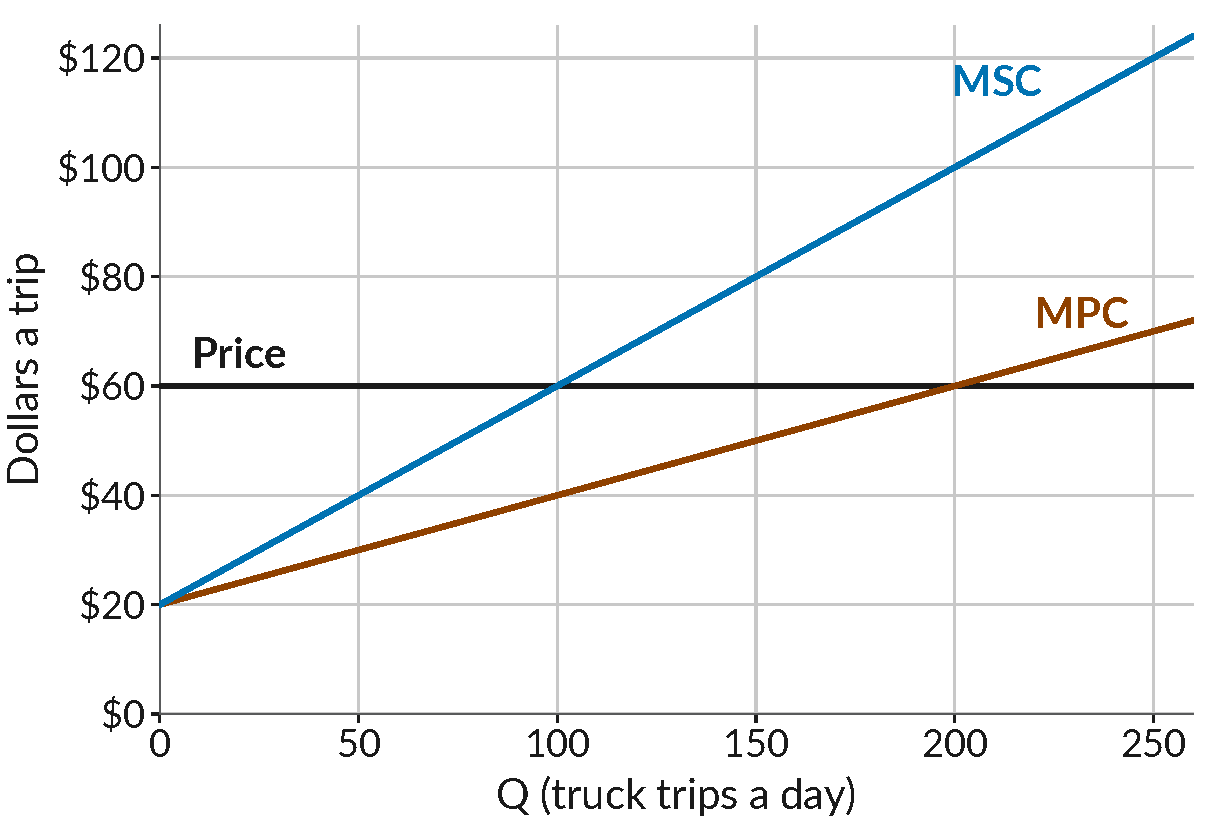
\includegraphics[width=0.6\textwidth, alt={A plotting grid, dollars a trip
on the vertical axis from 0 to 120 with gridlines every 20 dollars, and truck
trips a day on the horizontal axis from 0 to 250 with gridlines every 50
trips. The MPC line rises in a straight line from 20 dollars at zero trips to
40 dollars at 100 trips and 60 dollars at 200 trips. The MSC line starts at
the same point and rises twice as fast, from 20 dollars at zero trips to 60
dollars at 100 trips and 100 dollars at 200 trips. A horizontal line at 60
dollars is labelled Price.}]{figures/warehouse-grid.pdf}
\end{center}

\vspace{-18pt}
1. On the graph, mark the warehouse's choice (A) and the Pareto-efficient point (B). Label the trips.

\vspace{3pt}

2. \textbf{A cap.} The city caps trips at B. Compared with A, who gains and who loses?
\answerlines{2}

3. \textbf{A Pigouvian tax.} What is the MEC at B? What tax per trip gets the warehouse to B? Compared
with the cap, which does the warehouse prefer? Which do the neighbors prefer?
\answerlines{2}

4. \textbf{Compensation.} The warehouse must pay the neighbors the MEC of every trip. Why does it stop
at B? Which do the neighbors prefer, the tax or compensation?
\answerlines{2}

5. \textbf{Bargaining.} Suppose instead the neighbors bargain with the warehouse, which has the right
to run its trucks. Who pays whom? How does this differ from the three policies?
\answerlines{2}

\end{document}
